\documentclass[10pt]{article}

% A LaTeX reproduction of "Persecution of New Ideas" by C. L. Blood,
% as it appeared in Asher & Adams' New Columbian Rail Road Atlas and
% Pictorial Album of American Industry (1875):
% <http://www.davidrumsey.com/luna/servlet/detail/RUMSEY~8~1~35872~1201359:Persecution-of-New-Ideas---Dr--C-L-#>
%
% Typeset by Tristan Miller <http://www.nothingisreal.com/>
% November 2015
% 
% The article text and images are in the public domain.
% The LaTeX code is released under the Creative Commons
% Attribution 4.0 International (CC BY 4.0) licence.

% Page size, margins, and columns
\usepackage[
paperwidth=458mm,
paperheight=644mm,
left=36mm,
right=36mm,
top=52mm,
bottom=40mm
]{geometry}
\pagestyle{empty}
\usepackage{multicol}
\setlength\columnsep{10mm}
\setlength{\parindent}{8mm}
\def\columnseprulecolor{% Draw the column borders
\rotatebox{90}{\makebox[\textheight][c]{%
\rule{57mm}{0.7pt}%
\hfill
\rule{305mm}{0.7pt}%
}}}%

% Font and microtypography
\usepackage{lmodern}
\usepackage{microtype}
\usepackage[T1]{fontenc}

% Borders and figures
\usepackage{calc}
\usepackage{graphicx}
\usepackage{tikz}
\usetikzlibrary{calc}
\usepackage{eso-pic}
\usepackage{wrapfig}
\usepackage{wallpaper}
\definecolor{bordercolour}{RGB}{206,93,75}
\AddToShipoutPictureBG*{
  % Underlay the original document for tracing
  %\AtPageCenter{\makebox[0pt]{\raisebox{-.5\height}{%
  %\includegraphics[width=\pdfpagewidth]{blood_background}}}}%
  %
  % Draw the red page borders
  
\begin{tikzpicture}[overlay,remember picture]
    \draw[line width=3mm, color=bordercolour]
    ($ (current page.north west) + (26mm,-38mm) $)
    rectangle
    ($ (current page.south east) + (-26mm,26mm) $);
    \draw[line width=1.5pt, color=bordercolour]
    ($ (current page.north west) + (29mm,-41mm) $)
    rectangle
    ($ (current page.south east) + (-29mm,29mm) $);
  \end{tikzpicture}%
}

% PDF options
\usepackage{hyperref}
\hypersetup{
pdftitle={Persecution of New Ideas},
pdfauthor={C. L. Blood},
}

\begin{document}%
\TileWallPaper{0.5\textwidth}{0.5\textheight}{paper_background.jpg}%
\begin{multicols}{3}
% ----------------------------------------------------------------------
% First column
% ----------------------------------------------------------------------
\begin{centering}
\Large \scalebox{1.2}[1.0]{PERSECUTION OF NEW IDEAS.}

\vspace{3mm}

\rule[3pt]{2em}{0.7pt}

\vspace{2mm}

\large \scalebox{1.15}[1]{Dr.~C.~L.~Blood, Inventor of Oxygenized Air, for Diseases}\\[2.5mm]
\scalebox{1.15}[1]{of the Throat and Lungs.}

\vspace{3mm}

\rule[3pt]{2em}{0.7pt}

\vspace{2mm}

\end{centering}

\openup 1.09mm
When Christ appeared, and inculcated precepts superior to those of the\linebreak
Jewish teachers, he was persecuted for blasphemy. What the Jews could\linebreak
not overthrow by the learning of their priests, they sought to subdue by\linebreak
physical power. The treacherous sword of injustice was unsheathed\,;\linebreak
Jesus was wrongfully accused, condemned and crucified. His enemies\linebreak
believed their system of worship permanent and immutable, and treated him\linebreak
as a blasphemous impostor.

Abelard, for maintaining the rights of free inquiry, was condemned in\linebreak
solemn council. Farel, Lefevre, Hutton, Luther, Zwingle, Calvin, and a\linebreak
host of others, for lifting up the standard of independence, rejecting the in-\linebreak
fallibility of papacy, and condemning the unmeaning ceremony and\linebreak
legalized licentiousness of the church, were hunted down by mercenaries of\linebreak
the Pope, and menaced by the horrors of the Vatican. It was wrong for\linebreak
the human mind to assert its independence, and attempt to break loose from\linebreak
the restraints which had held the church and the world in darkness and\linebreak
degradation for centuries. Socrates taught the Athenians the existence of\linebreak
a supreme being, the source of all good, and the only true object of adora-\linebreak
tion. For this, he incurred the vengeance of those who should have ren-\linebreak
dered him gratitude, and was condemned to drink the juice of the hemlock.

When Descartes taught the doctrine of innate ideas he was declared an\linebreak
Atheist. The University of Paris became alarmed for the being of a God, and\linebreak
the purity of philosophy, and with all laudable zeal ordered the pestiferous\linebreak
works of the infidel author to be burned. It was but a short time, how-\linebreak
ever, till this same infallible University adopted the very doctrine it had\linebreak
combated so lustily, and when Locke and Coudillac attacked it, the cry of\linebreak
materialism and fatalism was turned against them. The teachings of Aris-\linebreak
totle were held for many years to be as permanent as the rock of truth.\linebreak
Francis I, passed a decree against Peter Raurno, interdicting him under\linebreak
pain of corporeal punishment, from uttering any more slanderous invectives\linebreak
against Aristotle, and other ancient authors, received and approved. About\linebreak
a century after, the Parliament of Paris passed a decree prohibiting any per-\linebreak
son, under pain of death, from holding or teaching any maxim at variance\linebreak
with the ancient and approved authors, especially the infallible Aristotle.\linebreak
More than a century after this, the medical faculty in Paris became alarmed\linebreak
for the safety of genuine medical science, and the Royal Academy of Medi-\linebreak
cine condemned inoculation as ``\,murderous, criminal and magical.'' Jen-\linebreak
ner was threatened with disgrace if he did not cease annoying the quietude\linebreak
and self-complacency of his friends with the silly visionary subject of vac-\linebreak
cination. Harvey for discovering the circulation of the blood, and an-\linebreak
nouncing the heretical fact, was treated with scorn by medical brethren, de-\linebreak
prived of his practice and driven into exile. It is a fact, containing an in-\linebreak
structive moral, that not one of his contemporaries at the age of forty years,\linebreak
when Harvey made known his discovery, ever conceded its correctness.\linebreak
They were stable-minded men and despised being led astray like boys by\linebreak
the glare of novelties. When Columbus made application to the Sovereigns\linebreak
of Europe for assistance in his project of western discovery, he met\linebreak
with cold neglect, and repeated repulse. The earth was as flat as a board,\linebreak
and how could he get to the East Indies by sailing west, and as to finding\linebreak
land, that was only the day dreams of a visionary madman. All the\linebreak
philosophy of the past was not to be capsized to suit the fantasy of an
\begin{wrapfigure}[36]{r}[.5\width+.5\columnwidth+\columnsep]{220mm}

\centering

\vspace{7mm}

\hspace{-6mm}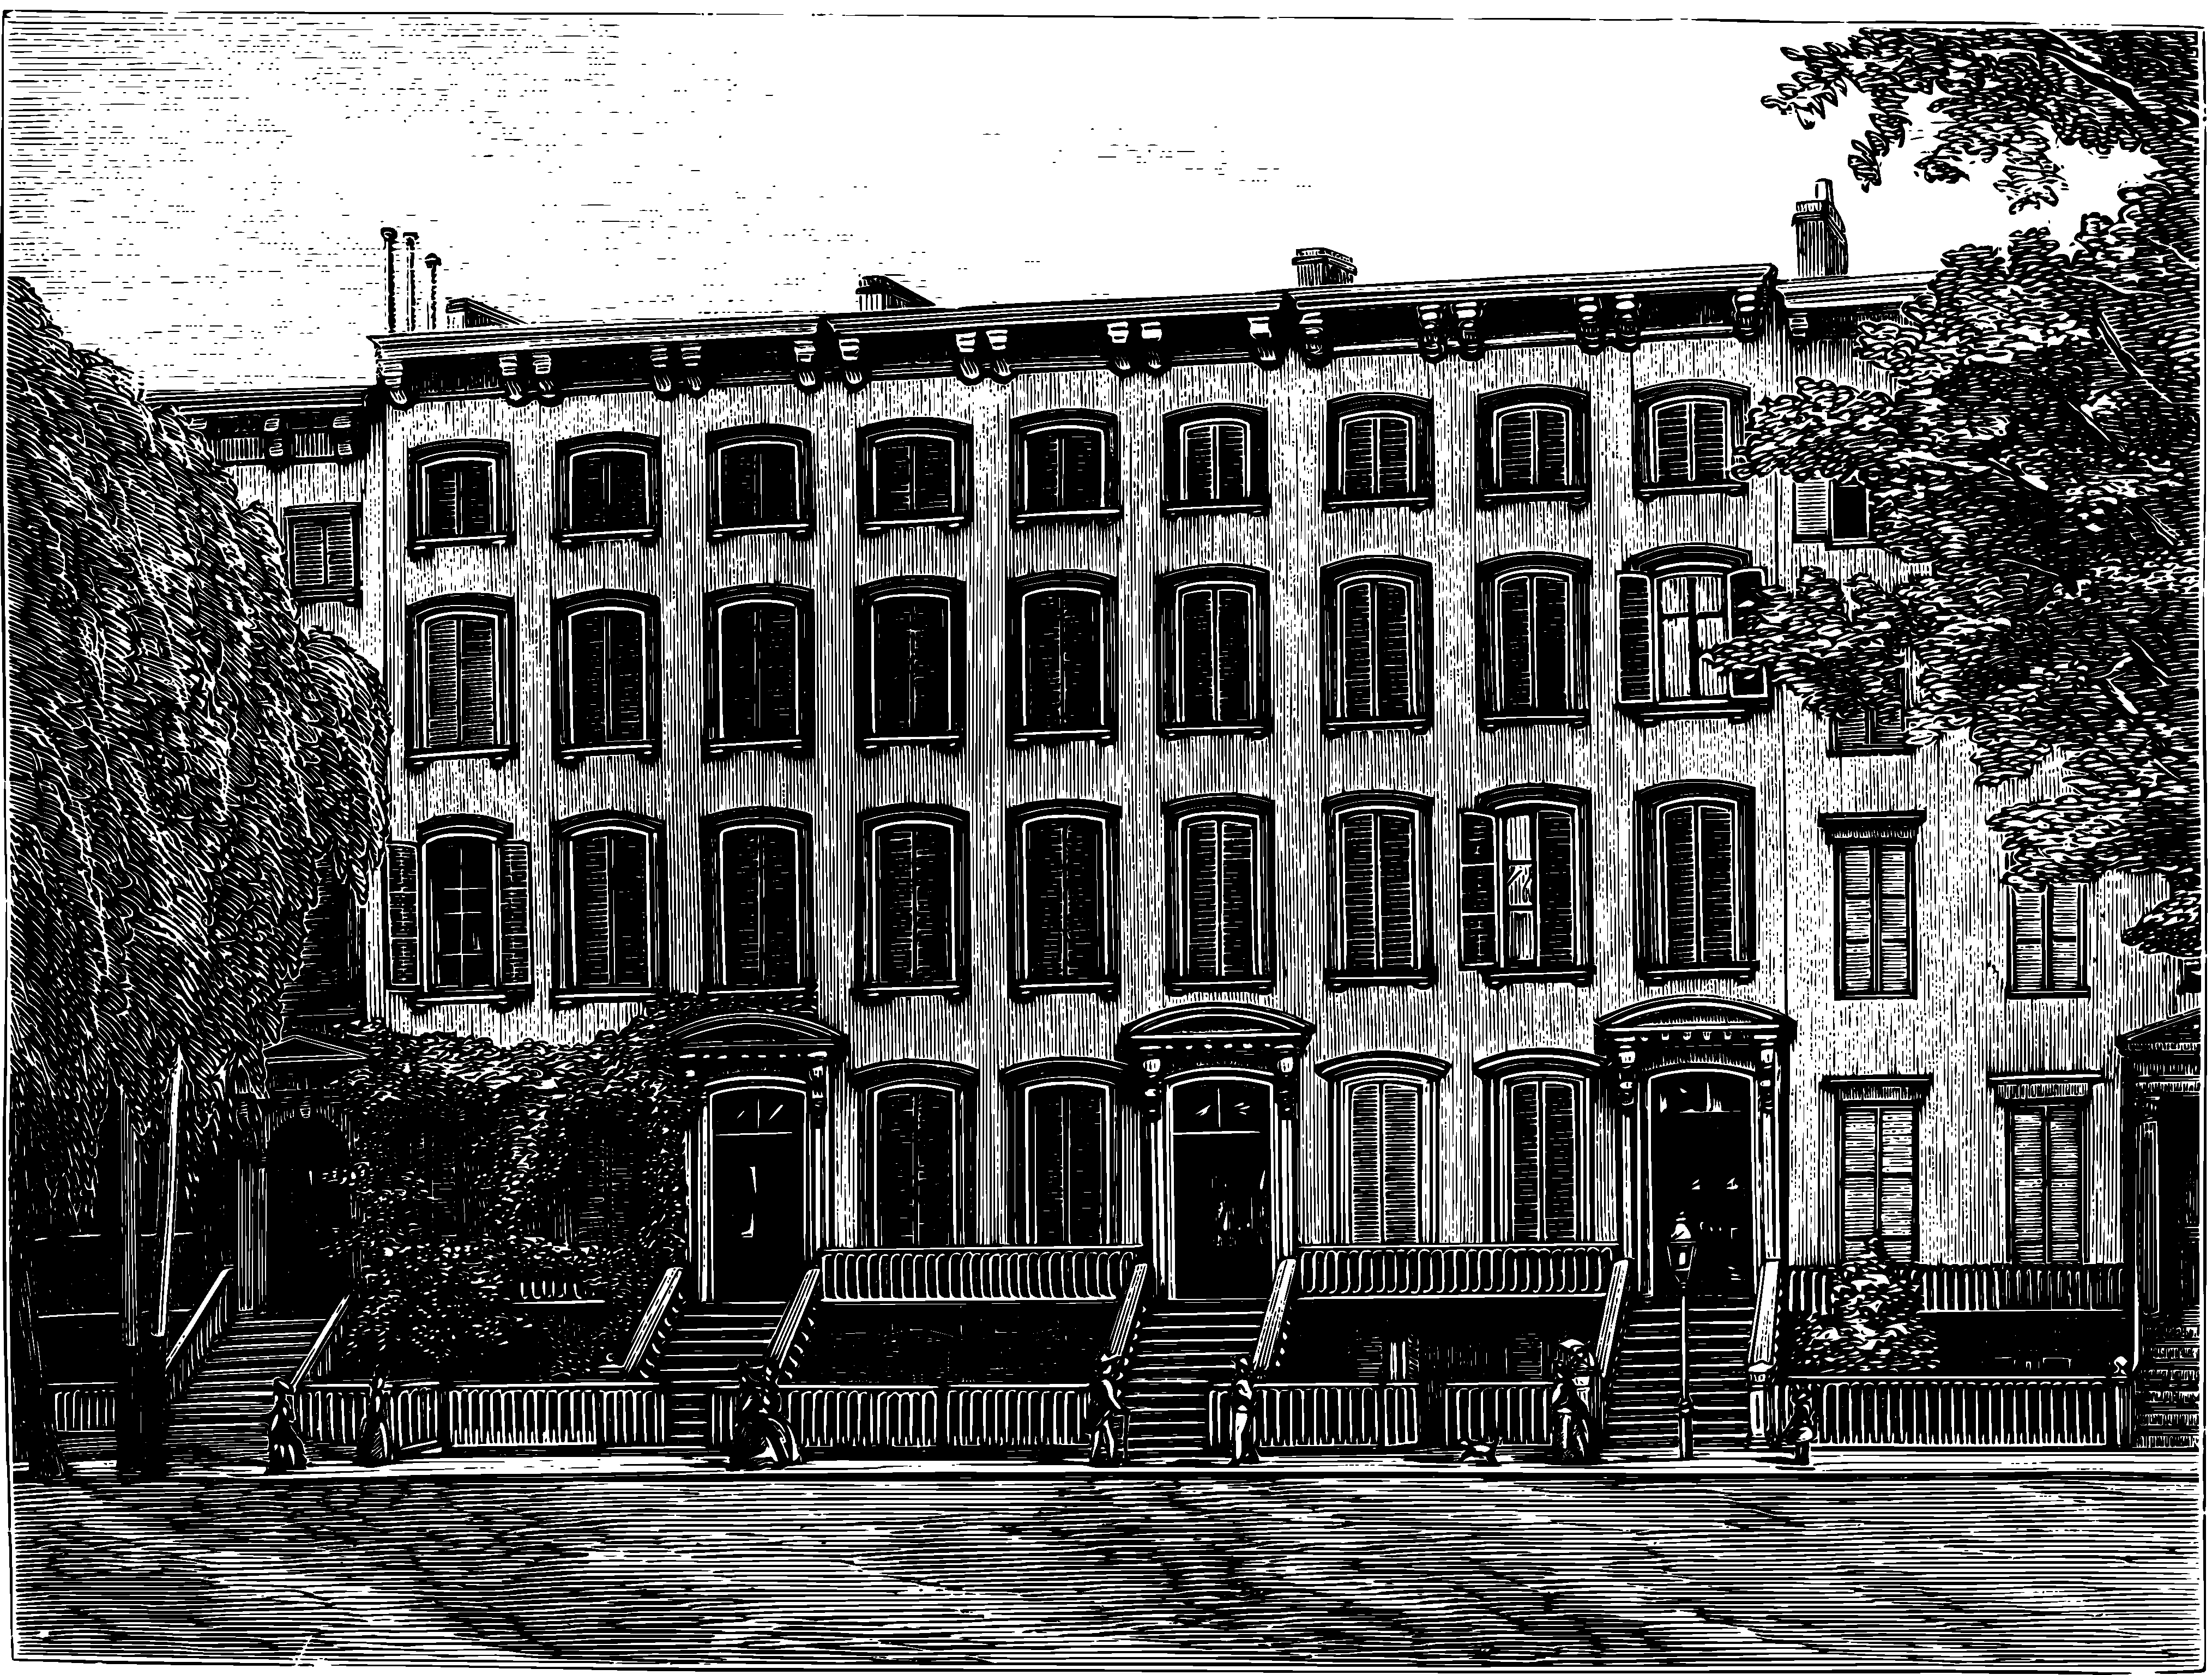
\includegraphics[width=207mm]{Office_and_residence_of_Dr_C_L_Blood.pdf}

\Large \hspace{-6mm}\scalebox{1.15}[1]{OFFICE AND RESIDENCE OF Dr.~C.~L.~BLOOD,}

\vspace{3mm}

\hspace{-8mm}\scalebox{1.15}[1]{27 Bond St.,\ near Broadway, New York City.}
\end{wrapfigure}
adventurer. When the persevering Fulton\linebreak
proposed to make steam a mighty agent in\linebreak
the propulsion of vessels, his capacious minded\linebreak
countrymen laughed at him. Steam had\linebreak
never propelled vessels\,; therefore it never\linebreak
could. The conclusion was as natural as to\linebreak
look to the past for all wisdom, and Fulton\linebreak
was ridiculed and neglected, and at last died\linebreak
in poverty.

From the introduction of Oxygenized Air,\linebreak
until the present time, the Old School has\linebreak
been lavish and unscrupulous in bestowing\linebreak
upon its author and those engaged in its ap-\linebreak
plication, the vilest vituperations. Knaves,\linebreak
fools, quacks and every degrading epithet\linebreak
which jealousy, ignorance and blind fanatical\linebreak
superstition could invent, have been applied\linebreak
to them.

Notwithstanding this great opposition,\linebreak
those engaged in the Oxygenized Air practice\linebreak
have calmly pursued their labors, and thou-\linebreak
sands of victims to the old school practice,\linebreak
who were on the verge of the grave, have been\linebreak
saved. Thousands who were on the road to\linebreak
eternity from consumption and other supposed\linebreak
incurable diseases, are to-day sound in body,\linebreak
and are living monuments to the worth of\linebreak
Oxygenized Air.

Dr.~Blood is one of the remarkable men\linebreak
of the age, of commanding presence, great\linebreak
intellectual attainments, a polished gentle-\linebreak
man, and is one of the most successful physi-\linebreak
cians in the country, if not in the world.

It is more than an eighth of a century\linebreak
since Dr.~Blood discovered a method for com-\linebreak
bining Oxygen and Nitrogen in such pro-\linebreak
portions as to make the Oxygen positively curative in its effects for diseases\linebreak
of the blood and lungs, and at the same time perfectly safe to inhale in any\linebreak
condition of health or disease.

When Dr.~Blood began to advocate the merits of his invention for the\linebreak
cure of diseases of the respiratory organs, he was met at the threshold of his\linebreak
career by a storm of derision and bitterness which would have driven an\linebreak
ordinary man from his purpose. His offence was that he dared to doubt\linebreak
the plenary inspirations and traditions of dead and rotten medical authors,\linebreak
whose errors were to be held as sacred as the living truths of Deity. War\linebreak
was declared, and the decree of social ostracism and defamatory rebuke was\linebreak
to silence the audacious innovator.\columnbreak

% ----------------------------------------------------------------------
% Second column
% ----------------------------------------------------------------------
There is scarce an exception to the rule that many who are so far in\linebreak
advance of the age in which they live, as to discover a new, or rather a be-\linebreak
fore unknown principle, for nothing is absolutely new, are generally re-\linebreak
viled.

Ambrose Pare introduced the ligature as a substitute for the painful\linebreak
mode of staunching the blood, after the amputation of a limb, viz: by ap-\linebreak
plying boiling pitch to the surface of the stump. He was, in consequence,\linebreak
persecuted with remorseless rancor by the Faculty, who ridiculed the idea\linebreak
of putting the life of a person upon a thread, when boiling pitch had stood\linebreak
the test for centuries. The Jesuits of Peru introduced the Peruvian\linebreak
Bark (invaluable as a medicine), but being a remedy used by the Jesuits,\linebreak
the Protestants at once rejected the drug as an invention of the devil.

\vspace{5mm}

\begin{centering}
\hspace{2mm}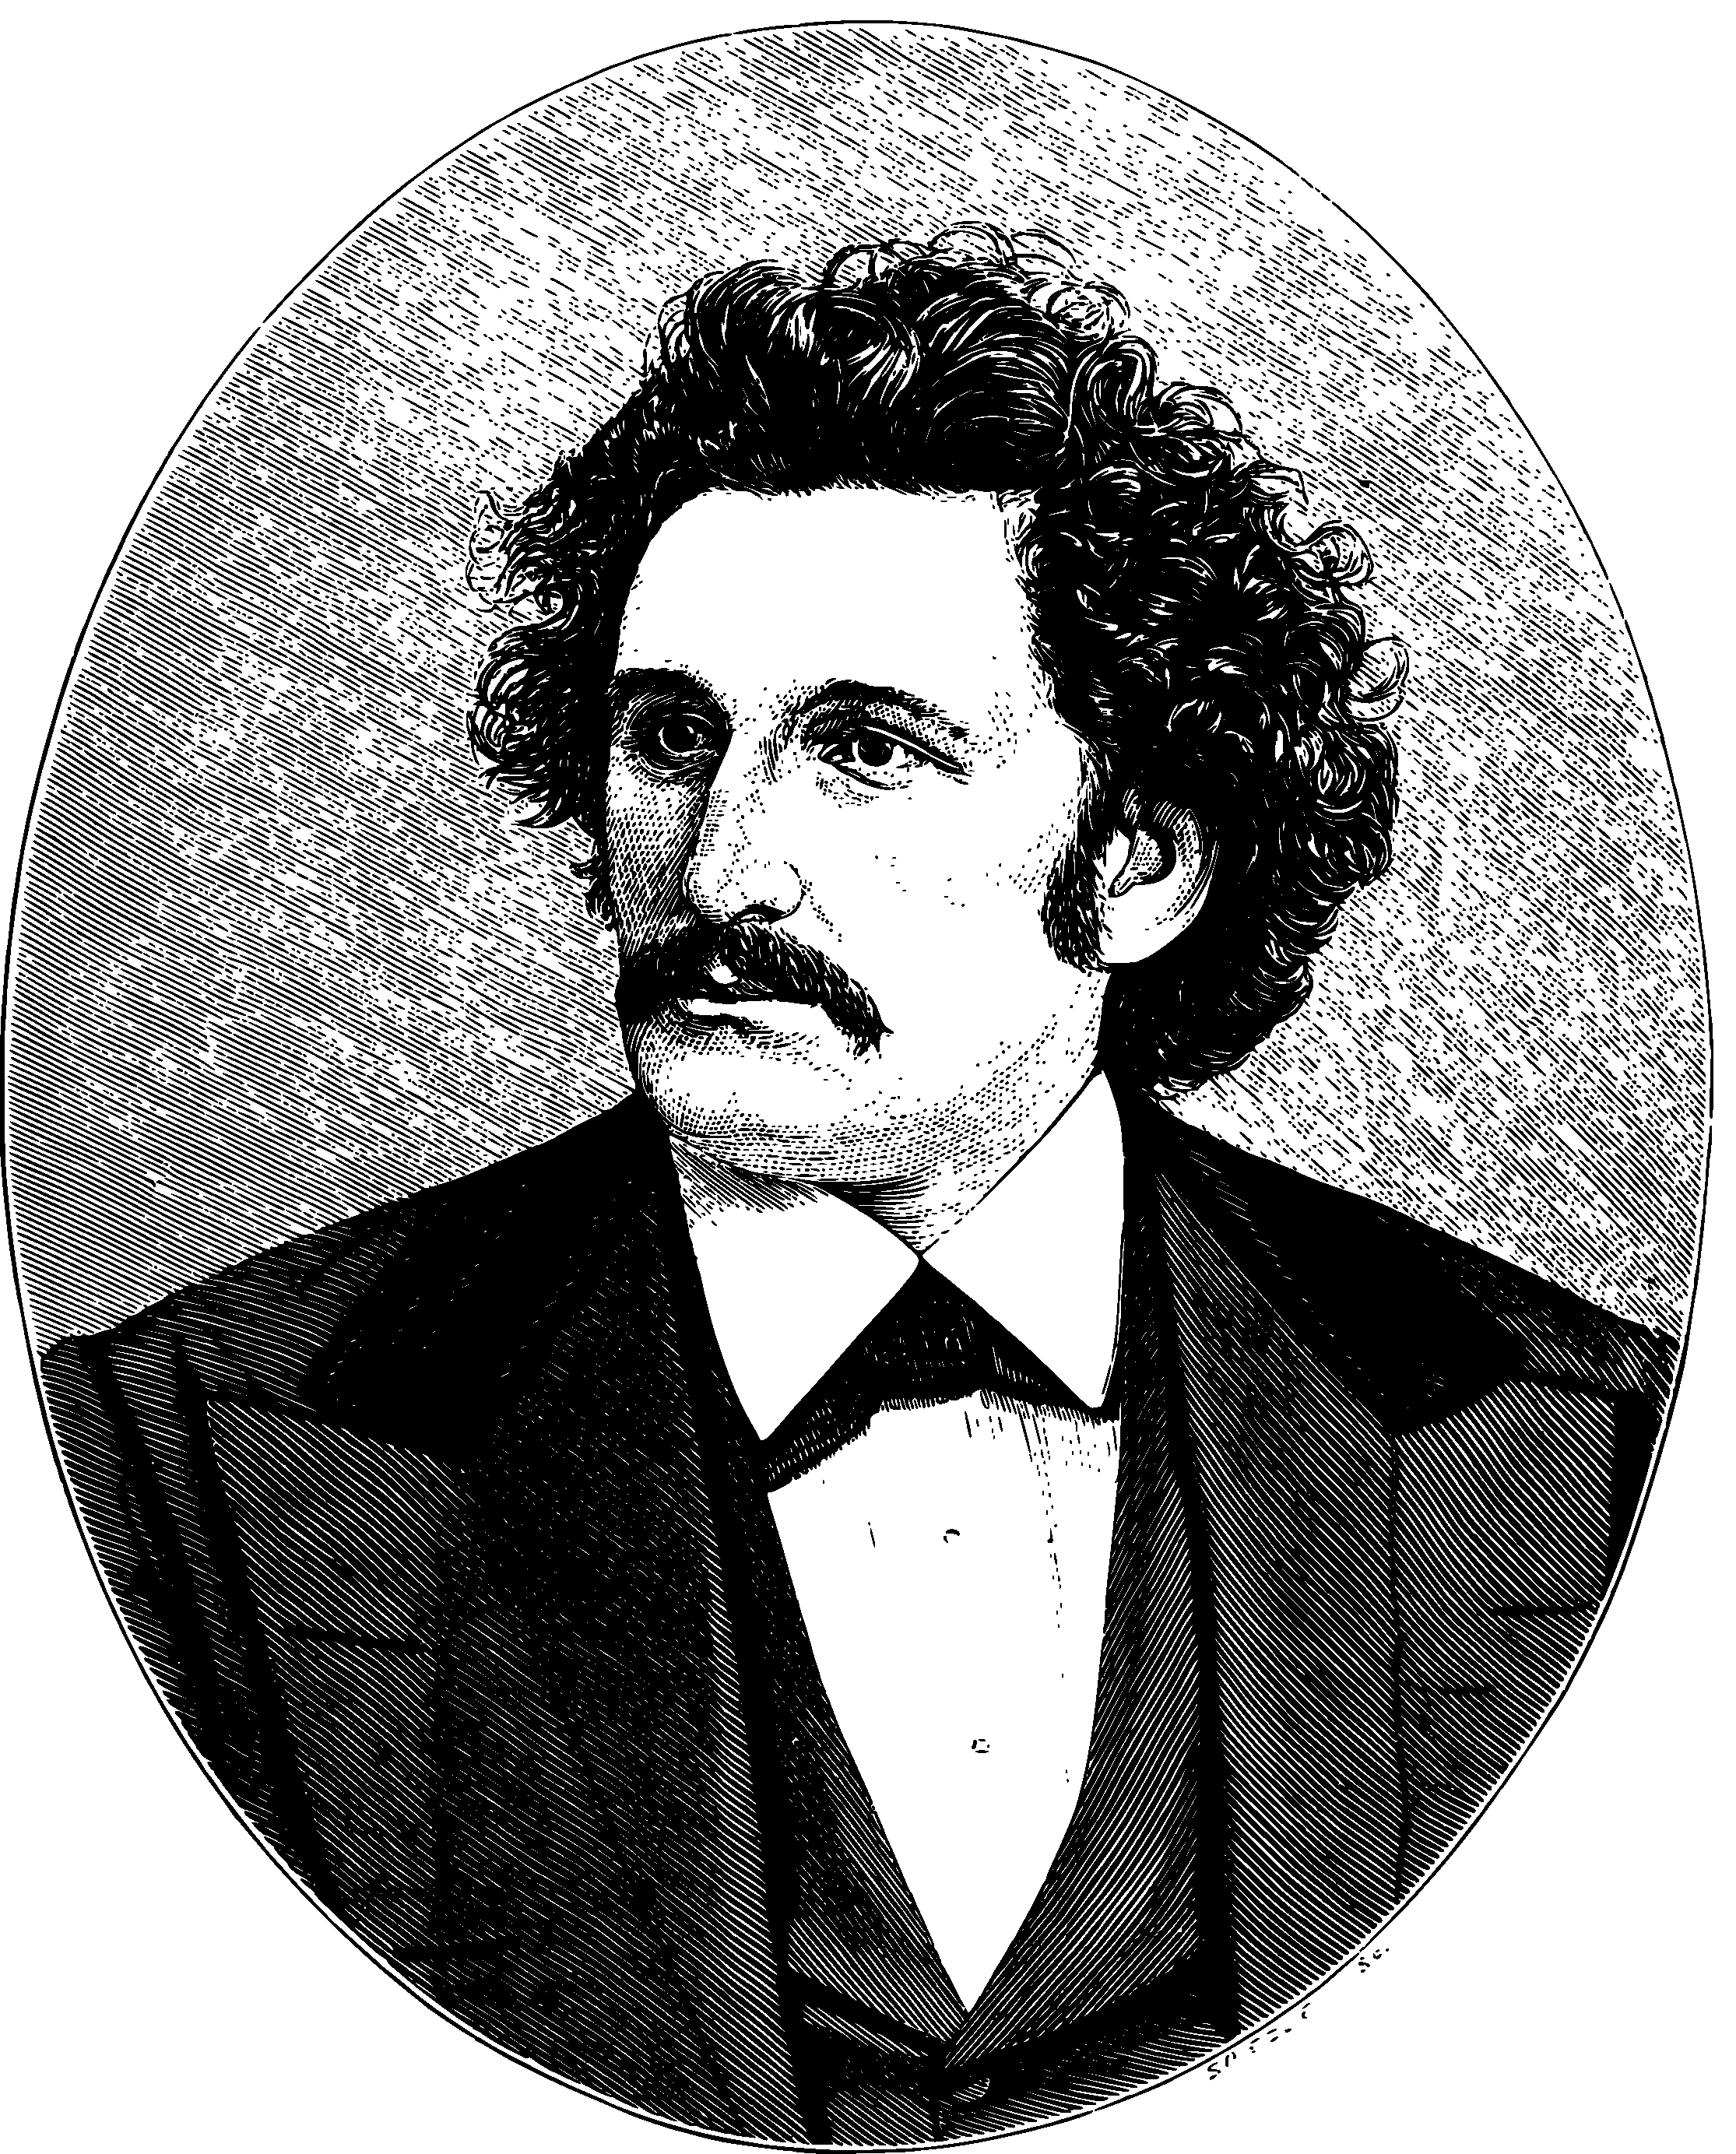
\includegraphics[width=112mm]{C_L_Blood.pdf}

\vspace{2mm}

\Large\scalebox{1.1}[1]{Dr.~C.~L.~BLOOD,}

\vspace{2.5mm}

\large\scalebox{1.2}[1]{Inventor of Oxygenized Air.}

\end{centering}

\vspace{2.75mm}

Dr.~Gronevelt discovered the curative power of Cantharides in Dropsy.\linebreak
As soon as his cures began to be noised abroad he was commited to New-\linebreak
gate by warrant of the President of the College of Physicians.

Physicians of the Old School have always been at war with progress,\linebreak
equal rights, and human liberty. The doctors have but recently secured\linebreak
the passage of a law by the legislature of New York, making it an offence\linebreak
punishable by fine and imprisonment for a physician or citizen to prescribe\linebreak
a medicine without first securing a license from them to do so. Their next\linebreak
effort will probably be to secure a law to prohibit the people from taking a\linebreak
medicine without a written order from some member of the faculty.

Notwithstanding the opposition of the bigoted and ignorant portion of\linebreak
the medical profession against Dr.~Blood in the introduction of his great dis-\linebreak
% ----------------------------------------------------------------------
% Third column
% ----------------------------------------------------------------------
covery, its grand principle remained impregnable, behind which he felt him-\linebreak
self secure and fortified against the assaults of a world of doctors, and he\linebreak

\vfill

\noindent persevered on until now his Oxygenized Air is almost universally acknow-\linebreak
ledged the most important medical discovery of the age. Over two hun-\linebreak
dred regular physicians have adopted it as a practice, and nearly every city\linebreak
in America, and many in Europe, have an office and a physician devoted\linebreak
to its application.

Dr.~Blood believes that if physicians of the old school would become\linebreak
less rigidly wedded to a dogmatic theory and system of treating diseases,\linebreak
suffering humanity would be greatly benefitted, He also believes that\linebreak
the rule of medical societies which does not allow its members to practice\linebreak
specialities, but compels them to treat all diseases, is productive of\linebreak
danger, suffering and death, as no physician is equally skillful in all dis-\columnbreak\linebreak
eases. He believes that this compulsory ``\,general practice'' destroys\linebreak
tens of thousands of lives every year. He also believes that the rule of\linebreak
medical societies which prohibits its members from advertising or making\linebreak
known to suffering humanity where they can be relieved or cured, is un-\linebreak
just and only calculated to gratify or benefit a few old fogy doctors who\linebreak
never should have been born. Dr.~Blood also believes that there is no\linebreak
science or safety in the old school practice. How far his views are sustained\linebreak
by medical men of character and note the following testimony will show.\linebreak
Notwithstanding medical men are very severe on quacks, it is impossible to\linebreak
look into medical literature without finding it replete with virtual confes-\linebreak
sions that medical men are immensely indebted to what they call quacks.

Radcliff said that ``\,when he died he would leave behind him the\linebreak
whole mystery of physics on half a sheet of paper.'' Sir Ashley Cooper is\linebreak
reported to have acknowledged that his ``\,mistakes would fill a church\linebreak
yard.'' Prof.~Jackson, of Philadelphia said that he ``\,would rather see a\linebreak
patient die than call in another doctor when such a step might appear to\linebreak
imply any distrust of his own abilities.''

One of the foremost English physicians and medical writers, Dr.\linebreak
James Johnson, says\,: ``\,I declare my conscientious opinion, founded on\linebreak
long observation and reflection, that if there was not a single physician,\linebreak
surgeon, apothecary, chemist, druggist or drug, on the face of the earth\linebreak
there would be less sickness and less mortality than now obtains.''

Prof.~Magendic addressed his students at the medical college at Paris\linebreak
as follows\,; ``\,Gentlemen, medicine is a great humbug. I know it is\linebreak
studied as a science. Doctors are mere imperics when they are not\linebreak
charlatans. We are as ignorant as men can be. Who knows anything in\linebreak
the world about medicine\,? There is no such thing as medical science. I\linebreak
grant you people are cured\,; but how\,? Nature does a great deal, imagin-\linebreak
ation does a great deal, doctors do devilish little.''

Dr.~O.~W.~Holmes says, ``\,Medicine is a grand colossal humbug.''\linebreak
There was a certain pope who lost his physician, and to all who applied for\linebreak
the office, he put the question, ``\,How many have you killed\,?'' Each\linebreak
doctor in turn solemnly asseverated that he had ``\,never killed anyone.''\linebreak
An old doctor, with a big beard, came at last. ``\,How many have you kill-\linebreak
ed\,?'' asked the pope. ``\,Two thousand,'' said the old fellow, pulling his\linebreak
beard with both hands. The pope was pleased with the confession, and,\linebreak
believing he must be a man of experience at least took him as his physician.

Statistics claimed to be authentic show a mortality under hom{\oe}opathy\linebreak
of about half---and in some diseases much less---than under allopathic\linebreak
treatment.

An allopathic physician in London sent to inspect the different cholera\linebreak
hospitals, concluded his report by avowing that, ``\,if taken with the dis-\linebreak
ease, he desired hom{\oe}opathic treatment.''

It is an alleged fact that Hom{\oe}opathic Insurance Companies have\linebreak
about one-third the deaths on their hom{\oe}opathic policies that they do\linebreak
among the policy holders treated by allopathy---the actual fact being that\linebreak
they charge on the former a considerable less premium for the risk.\linebreak
Researches into the respective results of hom{\oe}opathic and allopathic private\linebreak
practice in New York City shows, for two years, thirty thousand three\linebreak
hundred and ninety-five deaths in the private practice of nine hundred and\linebreak
eighty-four allopathists and fifteen hundred and twenty in that of one\linebreak
hundred and fifty-six hom{\oe}opathists, showing fifty-three per cent. in favor\linebreak
of hom{\oe}opathy. Dr.~Blood advocates the hom{\oe}opathic treatment because\linebreak
if it does not always cure it does no harm.

Previous to Dr.~Blood's discovery of Oxygenized Air, he was engaged\linebreak
in the regular practice of medicine, prescribing for his patients from formu-\linebreak
las laid down in medical works, written by ignorant doctors who lived%\linebreak
\begin{wrapfigure}[36]{l}[.5\width+.5\columnwidth+\columnsep+4mm]{220mm}
\vfill
\end{wrapfigure}
before it was discovered that the blood circu-\linebreak
lated through the system, and which he was\linebreak
educated to believe would cure the various ills\linebreak
to which humanity are subject. But in many\linebreak
cases, in place of seeing his patients recover\linebreak
as he anticipated and expected, he saw them\linebreak
grow worse under the treatment called scien-\linebreak
tific, but which he found a curse and a\linebreak
delusion. Being a man of strong integrity,\linebreak
he abandoned the practice, feeling if he\linebreak
could not labor to promote the physical wel-\linebreak
fare of suffering mankind, he would not assist\linebreak
in entailing misery on the already myriads of\linebreak
victims to pernicious drugs.

Since Dr.~Blood commenced the Oxygen-\linebreak
ized Air practice he has treated personally\linebreak
over one hundred and twenty thousand\linebreak
patients, and in a majority of cases has ob-\linebreak
tained the finest results, restoring persons to\linebreak
health who had been drugged almost to death\linebreak
by other physicians and by them pronounced\linebreak
incurable. Unlike other physicians, Dr.\linebreak
Blood does not advise persons in the last\linebreak
stage of consumption to seek the air of the\linebreak
South or a trip across the briny deep, leaving\linebreak
home and kindred at the very time they most\linebreak
need their care, to risk their frail constitutions\linebreak
by perilous and exhausting journeys to far-off\linebreak
lands in pursuit of health\,; but, alas\,! where\linebreak
they too often meet with the sad fate of dying\linebreak
among strangers and in a strange land. If\linebreak
the disease in the lungs has not advanced too\linebreak
far, all the patient requires to regain his lost\linebreak
force and vitality is the soothing and puri-\linebreak
fying influence of Oxygenized Air, which,\linebreak
when taken into the lungs, sends the life\linebreak
blood gushing through the system and dyes their faded cheeks with the\linebreak
bloom of health.

What can be more natural, more simple and efficacious than the treat-\linebreak
ment of consumption by this method, by which the vital principle of life,\linebreak
Oxygen is conveyed directly into the lungs, and its life-giving properties\linebreak
brought to bear at once upon the seat of disease.

Dr.~Blood, enabled by this great discovery to alleviate the sick and\linebreak
suffering, must have reflected on his own soul the benign smiles of those he\linebreak
has been the means of benefiting and a gratiful people will hand down to\linebreak
posterity the blessed name of the one who gave to humanity the great\linebreak
boon of Oxygenized Air.
\end{multicols}
\end{document}

%%% Local Variables:
%%% mode: latex
%%% TeX-master: t
%%% End:
